\documentclass[10pt,aspectratio=169]{beamer}

% ==========================================
% Packages
% ==========================================
\usepackage{amsmath, amssymb}
\usepackage{tikz}
\usepackage{pgfplots}
\pgfplotsset{compat=1.17}
\usetikzlibrary{arrows.meta, positioning, shapes.geometric, decorations.pathreplacing, calc, fit, backgrounds}
\usepackage{listings}
\usepackage{xcolor}
\usepackage{booktabs}
\usepackage{adjustbox}
\usepackage{graphicx}
\usepackage{colortbl}
\usepackage{array}
\usepackage{multirow}

% Code listing style
\lstdefinestyle{cstyle}{
    backgroundcolor=\color{black!3},
    commentstyle=\color{green!50!black},
    keywordstyle=\color{blue!70!black}\bfseries,
    stringstyle=\color{red!70!black},
    basicstyle=\ttfamily\scriptsize,
    breakatwhitespace=false,
    breaklines=true,
    keepspaces=true,
    showspaces=false,
    showstringspaces=false,
    showtabs=false,
    tabsize=2,
    frame=single,
    framerule=0.2pt,
    rulecolor=\color{black!30},
    language=Python
}
\lstset{style=cstyle}

% ==========================================
% Color definitions
% ==========================================
\definecolor{ntnured}{RGB}{180, 0, 0}
\definecolor{ntnugrey}{RGB}{210, 210, 210}
\definecolor{titlebg}{RGB}{248, 248, 248}
\definecolor{itemblue}{RGB}{60, 60, 140}
\definecolor{accentblue}{RGB}{30, 80, 160}
\definecolor{accentgreen}{RGB}{30, 130, 80}
\definecolor{accentorange}{RGB}{220, 130, 30}
\definecolor{formulabg}{RGB}{240, 245, 255}
\definecolor{warnbg}{RGB}{255, 248, 220}

% ==========================================
% Theme
% ==========================================
\usetheme{Boadilla}
\usecolortheme[named=ntnured]{structure}
\useinnertheme[shadow]{rounded}

\setbeamercolor{title}{bg=titlebg, fg=ntnured}
\setbeamertemplate{title page}[default][rounded=true,shadow=true]
\setbeamertemplate{enumerate items}[ball]
\setbeamertemplate{itemize items}[ball]
\setbeamercolor{item projected}{bg=itemblue, fg=white}
\setbeamercolor{itemize item}{fg=itemblue}
\setbeamercolor{itemize subitem}{fg=itemblue!70}
\setbeamercolor{block title}{bg=ntnured!85, fg=white}
\setbeamercolor{block body}{bg=ntnured!5, fg=black}
\setbeamercolor{block title alerted}{bg=accentorange!85, fg=white}
\setbeamercolor{block body alerted}{bg=accentorange!8, fg=black}
\setbeamercolor{block title example}{bg=accentgreen!75, fg=white}
\setbeamercolor{block body example}{bg=accentgreen!8, fg=black}

% ==========================================
% Header
% ==========================================
\setbeamertemplate{headline}{
  \leavevmode%
  \hbox{%
  \begin{beamercolorbox}[wd=.5\paperwidth,ht=3ex,dp=1.25ex,left,leftskip=1em]{headline left}%
    \usebeamerfont{headline}\color{white}\textbf{\insertsectionhead}
  \end{beamercolorbox}%
  \begin{beamercolorbox}[wd=.5\paperwidth,ht=3ex,dp=1.25ex,right]{headline right}%
  \end{beamercolorbox}}%
  \vskip0pt%
}
\setbeamercolor{headline left}{bg=ntnured}
\setbeamercolor{headline right}{bg=ntnugrey}
\setbeamertemplate{navigation symbols}{}

% ==========================================
% Footer
% ==========================================
\setbeamertemplate{footline}{
  \leavevmode%
  \hbox{%
  \begin{beamercolorbox}[wd=.25\paperwidth,ht=2.25ex,dp=1ex,center]{author in head/foot}%
    \usebeamerfont{author in head/foot}\insertshortauthor
  \end{beamercolorbox}%
  \begin{beamercolorbox}[wd=.45\paperwidth,ht=2.25ex,dp=1ex,center]{title in head/foot}%
    \usebeamerfont{title in head/foot}\insertshorttitle
  \end{beamercolorbox}%
  \begin{beamercolorbox}[wd=.15\paperwidth,ht=2.25ex,dp=1ex,center]{date in head/foot}%
    \usebeamerfont{date in head/foot}\insertshortdate
  \end{beamercolorbox}%
  \begin{beamercolorbox}[wd=.15\paperwidth,ht=2.25ex,dp=1ex,right]{date in head/foot}%
    \insertframenumber{} / \inserttotalframenumber\hspace*{2ex}
  \end{beamercolorbox}}%
  \vskip0pt%
}

% ==========================================
% TikZ helper styles
% ==========================================
\tikzset{
  box/.style={rectangle, rounded corners=2pt, draw=ntnured!70, fill=ntnured!8,
              minimum height=0.9cm, minimum width=2.0cm, align=center, font=\scriptsize},
  bluebox/.style={rectangle, rounded corners=2pt, draw=accentblue!70, fill=accentblue!10,
              minimum height=0.9cm, minimum width=2.0cm, align=center, font=\scriptsize},
  greenbox/.style={rectangle, rounded corners=2pt, draw=accentgreen!70, fill=accentgreen!10,
              minimum height=0.9cm, minimum width=2.0cm, align=center, font=\scriptsize},
  flow/.style={-{Stealth[length=2mm]}, thick, draw=ntnured!70},
}

% ==========================================
% Title info
% ==========================================
\title[FGDS for Fast FIC]{CSC0071 Meta-heuristics and Problem Solving \\ Feature-Guided Domain Selection for Fast Fractal\\ Image Compression of High-Resolution Images}
\author[Wu, Lin, Ko]{
    \textmd{Course Instructor: Prof. Tsung-Che Chiang} \\
    \vspace{0.4cm}
    \textmd{Students: Zhen-Rong Wu, Darrin Lin, Liang-Yun Ko}}
\institute[NTNU]{
  Department of Computer Science and Information Engineering \\
  National Taiwan Normal University
}
\date[June 2026]{June 2026}

% ==========================================
\begin{document}
% ==========================================

% ---- Title ----
\begin{frame}
  \titlepage
\end{frame}

% ---- Outline ----
\section{Outline}
\begin{frame}{Outline}
  \begin{enumerate}
    \item \textbf{Background}: what is Fractal Image Compression (FIC), and why is it slow?
    \item \textbf{Motivation}: prior work uses PSO --- but it breaks at high resolution
    \item \textbf{The path to our method}: PSO $\to$ Memetic PSO $\to$ FG-PSO $\to$ the key ablation
    \item \textbf{FGDS}: feature extraction, KD-Tree candidate selection, exhaustive search
    \item \textbf{Genetic Algorithm}: learning which features matter
    \item \textbf{Experiments}: four connected experiments and what they prove
    \item \textbf{Conclusion} and contributions
  \end{enumerate}

  \vfill
  \begin{block}{One-sentence summary}
    We move the heuristic from \textbf{block matching} to \textbf{block selection}: instead of
    using a metaheuristic to \emph{match} blocks, we use features to \emph{select} a small,
    high-quality candidate pool, then search it exhaustively.
  \end{block}
\end{frame}

% ============================================================
\section{Background: Fractal Image Compression}
% ============================================================

\begin{frame}{What is Fractal Image Compression (FIC)?}
  \begin{columns}[T]
    \begin{column}{0.55\textwidth}
      \textbf{Core idea: an image is similar to itself at different scales.}
      \begin{itemize}
        \item A small \alert{range block} often looks like a shrunk, rotated copy of a larger
              region elsewhere in the image (a \alert{domain block}).
        \item Instead of storing pixels, we store \emph{instructions}: ``this block $=$ that
              region, shrunk, rotated, with contrast $s$ and brightness $o$.''
        \item These instructions form a set of \emph{contractive affine maps} (an Iterated
              Function System).
      \end{itemize}
      \vspace{0.2cm}
      \begin{block}{Why it is attractive}
        \begin{itemize}
          \item High compression ratio.
          \item \textbf{Resolution-independent} decoding: zoom in without blocking artifacts.
        \end{itemize}
      \end{block}
    \end{column}
    \begin{column}{0.45\textwidth}
      \centering
      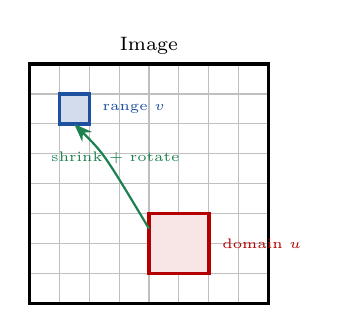
\begin{tikzpicture}[scale=0.95]
        % big image grid
        \draw[step=0.4cm, gray!50, thin] (0,0) grid (3.2,3.2);
        \draw[very thick, black] (0,0) rectangle (3.2,3.2);
        \node[font=\scriptsize] at (1.6,3.45) {Image};
        % a range block (small)
        \draw[very thick, accentblue, fill=accentblue!20] (0.4,2.4) rectangle (0.8,2.8);
        \node[accentblue, font=\tiny, right] at (0.85,2.6) {range $v$};
        % a domain block (large)
        \draw[very thick, ntnured, fill=ntnured!10] (1.6,0.4) rectangle (2.4,1.2);
        \node[ntnured, font=\tiny, right] at (2.45,0.8) {domain $u$};
        % arrow showing the map
        \draw[-{Stealth}, thick, accentgreen]
            (1.6,1.0) .. controls (1.0,2.0) .. (0.6,2.4);
        \node[accentgreen, font=\tiny] at (1.15,1.95) {shrink + rotate};
      \end{tikzpicture}
      \vspace{0.3cm}
      \[
        \hat v = s\cdot T_k(\text{downsample}(u)) + o
      \]
      {\scriptsize $T_k$: one of 8 rotations/flips; $s$: contrast; $o$: brightness.}
    \end{column}
  \end{columns}
\end{frame}

\begin{frame}{Encoding vs.\ decoding: the asymmetry}
  \begin{columns}[T]
    \begin{column}{0.5\textwidth}
      \begin{block}{Decoding is \textcolor{accentgreen}{fast}}
        Start from \emph{any} image, repeatedly apply the stored maps. By Banach's
        fixed-point theorem it converges to a unique reconstruction in $\sim$20 iterations.
      \end{block}
      \begin{alertblock}{Encoding is \textcolor{ntnured}{slow}}
        For \textbf{every} range block we must find the \textbf{best} domain block and isometry:
        \[
          \min_{u\in\mathcal D,\; k\in\{0..7\}} \text{MSE}\big(v,\; s\,T_k(u)+o\big)
        \]
        $s,o$ have a closed form; the hard part is the \emph{search} over $u$ and $k$.
      \end{alertblock}
    \end{column}
    \begin{column}{0.5\textwidth}
      \textbf{The cost explodes with resolution.}
      \begin{itemize}
        \item For a $1024\times1024$ image with $4\times4$ range blocks:
        \begin{itemize}
          \item[] $M = 65{,}536$ range blocks
          \item[] $P = 65{,}025$ domain blocks
          \item[] $\times\, 8$ isometries
        \end{itemize}
        \item Full search $=$ $M\times P\times 8 \approx \mathbf{3.4\times 10^{10}}$
              evaluations \emph{per image}.
      \end{itemize}
      \vspace{0.2cm}
      \begin{block}{The research question}
        Can we keep the quality of full search while drastically cutting this cost?
      \end{block}
    \end{column}
  \end{columns}
\end{frame}

\begin{frame}{One ``fitness evaluation'' (FFE) --- the unit of cost}
  \begin{columns}[T]
    \begin{column}{0.58\textwidth}
      For a fixed range block $v$, domain block $u$, and isometry $k$, the optimal contrast
      and brightness have a \textbf{closed-form least-squares solution}:
      \[
        s = \frac{\text{Cov}(v,u_k)}{\text{Var}(u_k)}, \qquad o = \bar v - s\,\bar u_k,
      \]
      \[
        \text{MSE} = \tfrac{1}{L^2}\textstyle\sum (v - s\,u_k - o)^2 .
      \]
      \begin{itemize}
        \item One such computation $=$ one \alert{Fitness Function Evaluation (FFE)}.
        \item \textbf{Every} method in this talk is measured in FFEs --- this makes the
              comparison fair.
        \item Contractivity $|s|<1$ is required for the decoder to converge.
      \end{itemize}
    \end{column}
    \begin{column}{0.42\textwidth}
      \begin{block}{Key observation we will exploit}
        \begin{itemize}
          \item A \textbf{mean} mismatch ($\bar v\!\neq\!\bar u$) is absorbed \emph{exactly}
                by the offset $o$ --- it costs nothing.
          \item A \textbf{contrast} mismatch ($\sigma_v\!\neq\!\sigma_u$) cannot be absorbed
                --- it directly inflates the MSE.
        \end{itemize}
        $\Rightarrow$ Standard deviation matters far more than mean for choosing a good
        domain. (We will let a GA discover this.)
      \end{block}
    \end{column}
  \end{columns}
\end{frame}

% ============================================================
\section{Motivation: PSO and Why It Breaks}
% ============================================================

\begin{frame}{Prior work: replace the search with a metaheuristic}
  \begin{columns}[T]
    \begin{column}{0.55\textwidth}
      \textbf{The standard approach} (Muruganandham \& Wahida Banu, 2010):
      treat $(d, k)$ --- domain index and isometry --- as the variables, and search
      with \alert{Particle Swarm Optimization (PSO)}.
      \begin{itemize}
        \item Each particle $=$ a candidate $(d,k)$.
        \item Particles fly through the search space, pulled toward their own best
              and the swarm's global best.
      \end{itemize}
      \[
        \mathbf V \leftarrow w\mathbf V + c_1 r_1(\mathbf P_{best}-\mathbf X)
                                       + c_2 r_2(\mathbf G_{best}-\mathbf X)
      \]
      Genetic algorithms and pyramid-PSO have also been tried in the same spirit.
    \end{column}
    \begin{column}{0.45\textwidth}
      \begin{alertblock}{The problem at high resolution}
        \begin{itemize}
          \item One range block has $P\times 8 \approx \mathbf{5.2\times 10^5}$ candidates.
          \item A swarm of 40 particles covers $<0.01\%$ of that at start.
          \item The objective over domain indices is \emph{not smooth}: neighboring
                domains can be totally different.
          \item $\Rightarrow$ the swarm has no gradient to follow and gets stuck far from
                the optimum.
        \end{itemize}
      \end{alertblock}
      \textbf{Our diagnosis:} the weakness is not the optimizer --- it is the
      \textbf{quality of the search space} we hand it.
    \end{column}
  \end{columns}
\end{frame}

% ============================================================
\section{The Path to Our Method}
% ============================================================

\begin{frame}{Our reasoning trail (each step is an experiment)}
  \centering
  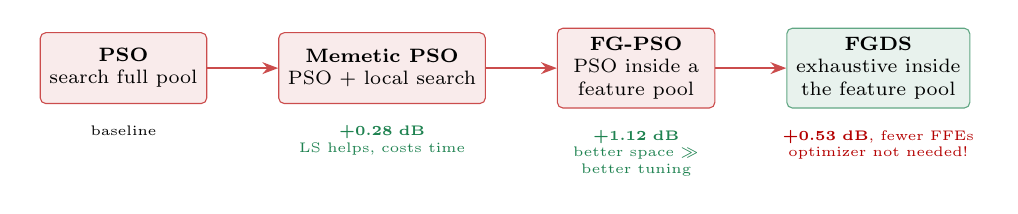
\begin{tikzpicture}[node distance=0.45cm and 0.9cm]
    \node[box] (pso) {\textbf{PSO}\\ search full pool};
    \node[box, right=of pso] (mpso) {\textbf{Memetic PSO}\\ PSO $+$ local search};
    \node[box, right=of mpso] (fgpso) {\textbf{FG-PSO}\\ PSO inside a\\ feature pool};
    \node[greenbox, right=of fgpso] (fgds) {\textbf{FGDS}\\ exhaustive inside\\ the feature pool};

    \draw[flow] (pso) -- (mpso);
    \draw[flow] (mpso) -- (fgpso);
    \draw[flow] (fgpso) -- (fgds);

    \node[below=0.15cm of pso, font=\tiny, text width=2.2cm, align=center] {baseline};
    \node[below=0.15cm of mpso, font=\tiny, text width=2.4cm, align=center, accentgreen]
        {\textbf{+0.28 dB}\\ LS helps, costs time};
    \node[below=0.15cm of fgpso, font=\tiny, text width=2.4cm, align=center, accentgreen]
        {\textbf{+1.12 dB}\\ better space $\gg$ better tuning};
    \node[below=0.15cm of fgds, font=\tiny, text width=2.6cm, align=center, ntnured]
        {\textbf{+0.53 dB}, fewer FFEs\\ optimizer not needed!};
  \end{tikzpicture}

  \vspace{0.5cm}
  \begin{columns}
    \begin{column}{0.92\textwidth}
      \begin{block}{The decisive insight}
        Once the candidate pool is small (a few hundred), \textbf{exhaustive search beats PSO}
        inside it --- it is exact, deterministic, and uses fewer evaluations. So we
        \textbf{remove the metaheuristic matcher} and keep only the feature-guided
        \emph{selection}. That selection becomes our contribution.
      \end{block}
    \end{column}
  \end{columns}
\end{frame}

\begin{frame}{The three baselines, briefly}
  \begin{block}{1. Standard PSO}
    A swarm of 40 particles searches the full $(d,k)$ space. Cheap per step, but lost in a
    huge space.
  \end{block}
  \begin{block}{2. Memetic PSO ($=$ PSO $+$ local search)}
    Every few iterations, refine the best particles:
    \begin{itemize}
      \item \textbf{Isometry-LS}: try the other 7 isometries of the current domain.
      \item \textbf{Spatial-LS}: try the 8 spatially adjacent domain blocks.
    \end{itemize}
    \emph{Lesson:} local search reliably raises PSNR --- but adds time.
  \end{block}
  \begin{block}{3. Feature-Guided PSO (FG-PSO)}
    First build a small feature-based candidate pool (top-$K$ domains per range block), then
    run Memetic PSO \emph{inside} that pool. \emph{Lesson:} shrinking the space to high-quality
    candidates helps much more than tuning the optimizer.
  \end{block}
\end{frame}

% ============================================================
\section{Proposed Method: FGDS}
% ============================================================

\begin{frame}{FGDS pipeline: select first, then search}
  \centering
  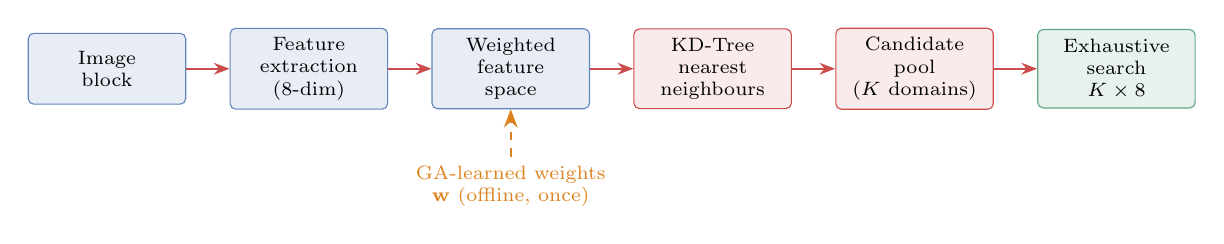
\begin{tikzpicture}[node distance=0.35cm and 0.55cm]
    \node[bluebox] (img) {Image\\ block};
    \node[bluebox, right=of img] (feat) {Feature\\ extraction\\ (8-dim)};
    \node[bluebox, right=of feat] (wfs) {Weighted\\ feature\\ space};
    \node[box, right=of wfs] (kd) {KD-Tree\\ nearest\\ neighbours};
    \node[box, right=of kd] (pool) {Candidate\\ pool\\ ($K$ domains)};
    \node[greenbox, right=of pool] (exh) {Exhaustive\\ search\\ $K\times 8$};

    \draw[flow] (img)--(feat);
    \draw[flow] (feat)--(wfs);
    \draw[flow] (wfs)--(kd);
    \draw[flow] (kd)--(pool);
    \draw[flow] (pool)--(exh);

    \node[below=0.6cm of wfs, font=\scriptsize, accentorange, text width=3cm, align=center]
        (ga) {GA-learned weights $\mathbf w$ (offline, once)};
    \draw[-{Stealth}, thick, accentorange, dashed] (ga) -- (wfs);
  \end{tikzpicture}

  \vspace{0.4cm}
  \begin{columns}[T]
    \begin{column}{0.5\textwidth}
      \begin{block}{Three online stages}
        \begin{enumerate}
          \item Describe every block by 8 numbers.
          \item Use a KD-Tree to find the $K$ most similar domains per range block.
          \item Exhaustively try those $K\times 8$ candidates; keep the best.
        \end{enumerate}
      \end{block}
    \end{column}
    \begin{column}{0.5\textwidth}
      \begin{exampleblock}{Why this is fast \emph{and} good}
        \begin{itemize}
          \item Search space per block: $520{,}200 \to 640$ ($K{=}80$).
          \item Exhaustive within the pool $\Rightarrow$ optimal, deterministic.
          \item Selection is structure-aware $\Rightarrow$ the pool already contains good
                matches.
        \end{itemize}
      \end{exampleblock}
    \end{column}
  \end{columns}
\end{frame}

\begin{frame}{Stage 1: an 8-dimensional isometry-invariant descriptor}
  \begin{columns}[T]
    \begin{column}{0.52\textwidth}
      Each block $b$ ($L\times L$) becomes a vector:
      \[
        \mathbf f(b)=[\,\underbrace{\mu,\sigma}_{\text{intensity}},\;
                       \underbrace{\bar g_h,\bar g_v}_{\text{texture}},\;
                       \underbrace{\hat q_1,\hat q_2,\hat q_3,\hat q_4}_{\text{layout (sorted)}}\,]
      \]
      \begin{itemize}
        \item $\mu,\sigma$: mean \& standard deviation.
        \item $\bar g_h,\bar g_v$: mean horizontal/vertical gradient magnitude (texture).
        \item $\hat q_{1..4}$: the four quadrant means, \alert{sorted ascending}.
      \end{itemize}
      \begin{block}{Two requirements}
        \textbf{Discriminative} (separates different blocks) \\
        \textbf{Isometry-invariant}: a domain under any rotation/flip is the \emph{same}
        candidate (the isometry is searched later, in Stage 3).
      \end{block}
    \end{column}
    \begin{column}{0.48\textwidth}
      \centering
      \textbf{Why sorting the quadrants gives invariance}
      \vspace{0.2cm}

      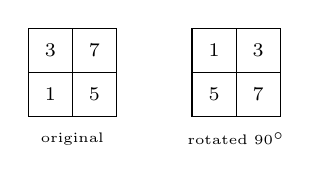
\begin{tikzpicture}[scale=0.8]
        % original
        \draw (0,0) rectangle (1.4,1.4);
        \draw (0.7,0)--(0.7,1.4); \draw (0,0.7)--(1.4,0.7);
        \node[font=\scriptsize] at (0.35,1.05){3}; \node[font=\scriptsize] at (1.05,1.05){7};
        \node[font=\scriptsize] at (0.35,0.35){1}; \node[font=\scriptsize] at (1.05,0.35){5};
        \node[font=\tiny, below] at (0.7,-0.1){original};
        % rotated
        \begin{scope}[xshift=2.6cm]
          \draw (0,0) rectangle (1.4,1.4);
          \draw (0.7,0)--(0.7,1.4); \draw (0,0.7)--(1.4,0.7);
          \node[font=\scriptsize] at (0.35,1.05){1}; \node[font=\scriptsize] at (1.05,1.05){3};
          \node[font=\scriptsize] at (0.35,0.35){5}; \node[font=\scriptsize] at (1.05,0.35){7};
          \node[font=\tiny, below] at (0.7,-0.1){rotated 90$^\circ$};
        \end{scope}
      \end{tikzpicture}

      \vspace{0.3cm}
      Quadrant values are \emph{permuted} by rotation, but
      \[
        \text{sort}(3,7,1,5)=\text{sort}(1,3,5,7)=(1,3,5,7)
      \]
      \alert{same vector} $\Rightarrow$ fully invariant.
      \vspace{0.2cm}

      Features are $z$-score normalized so each dimension is comparable.
    \end{column}
  \end{columns}
\end{frame}

\begin{frame}{What is a KD-Tree?}
  \begin{columns}[T]
    \begin{column}{0.5\textwidth}
      A \alert{KD-Tree} is a binary tree that recursively splits points along alternating
      coordinate axes. It answers ``\textbf{which points are nearest to this query?}'' in
      $O(\log P)$ instead of $O(P)$.
      \begin{itemize}
        \item Split the data by the $x$-median, then each half by the $y$-median, and so on.
        \item To find neighbours, descend to the query's leaf and prune branches that are
              provably too far.
        \item Efficient in low dimensions (our space is only 8-D; trouble starts above $\sim$20).
      \end{itemize}
      \begin{block}{In our project}
        Points $=$ the 8-D feature vectors of all $P$ \textbf{domain} blocks.
        Query $=$ a \textbf{range} block's feature vector.
        Answer $=$ its $K$ nearest domains.
      \end{block}
    \end{column}
    \begin{column}{0.5\textwidth}
      \centering
      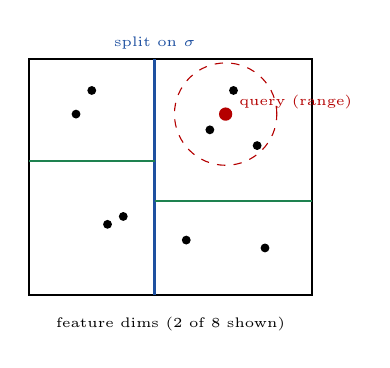
\begin{tikzpicture}[scale=1.0]
        % 2D space with splits (illustrative, 2 of the 8 dims)
        \draw[thick] (0,0) rectangle (3.6,3.0);
        % first split vertical
        \draw[accentblue, very thick] (1.6,0)--(1.6,3.0);
        \node[accentblue, font=\tiny, above] at (1.6,3.0){split on $\sigma$};
        % second splits horizontal
        \draw[accentgreen, thick] (0,1.7)--(1.6,1.7);
        \draw[accentgreen, thick] (1.6,1.2)--(3.6,1.2);
        % points
        \foreach \p in {(0.6,2.3),(1.0,0.9),(0.8,2.6),(1.2,1.0),
                        (2.3,2.1),(3.0,0.6),(2.6,2.6),(2.9,1.9),(2.0,0.7)}
          \fill[black] \p circle (1.6pt);
        % query
        \fill[ntnured] (2.5,2.3) circle (2.4pt);
        \node[ntnured, font=\tiny, right] at (2.55,2.45){query (range)};
        % nearest circle
        \draw[ntnured, dashed] (2.5,2.3) circle (0.65cm);
        \node[font=\tiny, below] at (1.8,-0.15){feature dims (2 of 8 shown)};
      \end{tikzpicture}

      \vspace{0.25cm}
      {\scriptsize The dashed circle is the $K$-nearest region; the tree lets us find it
      without scanning all points.}
    \end{column}
  \end{columns}
\end{frame}

\begin{frame}{How we use the KD-Tree on domain features}
  \begin{columns}[T]
    \begin{column}{0.5\textwidth}
      \textbf{The matching distance is weighted Euclidean:}
      \[
        \mathcal P_i=\operatorname*{arg\,min}_{|S|=K}\sum_{j\in S}
          \big\| \mathbf w \odot (\hat{\mathbf f}_{R,i}-\hat{\mathbf f}_{D,j})\big\|^2
      \]
      \textbf{Trick:} pre-multiply \emph{both} range and domain features by $\mathbf w$.
      Then weighted distance $=$ plain Euclidean distance $\Rightarrow$ a standard KD-Tree
      works directly.
      \vspace{0.2cm}
      \begin{enumerate}
        \item Build one KD-Tree from all $P$ weighted domain features.
        \item Batch-query all $M$ range features at once for their top-$K$.
      \end{enumerate}
    \end{column}
    \begin{column}{0.5\textwidth}
      \begin{exampleblock}{The speedup that motivated this}
        Pairwise (brute-force) pool construction:
        \[
          O(M\cdot P\cdot F)\;\approx\; \mathbf{180\ s}
        \]
        KD-Tree pool construction:
        \[
          O(P F\log P + M K\log P)\;<\;\mathbf{0.5\ s}
        \]
        \centering \alert{$\approx 1390\times$ faster, identical result.}
      \end{exampleblock}
      \begin{block}{Important}
        The KD-Tree returns the \textbf{same} neighbours as brute force --- so PSNR is
        \emph{unchanged}. Only the time changes.
      \end{block}
    \end{column}
  \end{columns}
\end{frame}

\begin{frame}{Stage 3: exhaustive search inside the pool}
  \begin{columns}[T]
    \begin{column}{0.55\textwidth}
      For each range block, we now have only $K$ candidate domains. We try \textbf{all}
      $K\times 8$ (domain, isometry) pairs and keep the one with minimum MSE
      (subject to $|s|<1$).
      \begin{itemize}
        \item With $K=80$: $640$ FFEs per block.
        \item This is \emph{fewer} than the budget given to the PSO baselines.
        \item Yet it is \textbf{exact} within the pool and fully \textbf{deterministic} ---
              no random restarts, no tuning.
      \end{itemize}
    \end{column}
    \begin{column}{0.45\textwidth}
      \begin{block}{Why not PSO here?}
        In a 640-candidate space, PSO would (a) round continuous positions to indices and
        possibly skip candidates, and (b) need multiple runs for stability. A complete scan
        is simply better --- this is the ablation that let us drop the optimizer.
      \end{block}
      \begin{alertblock}{Cost reduction vs.\ full search}
        $3.4\times10^{10} \to 4.2\times10^{7}$ FFEs/image
        ($>800\times$ fewer).
      \end{alertblock}
    \end{column}
  \end{columns}
\end{frame}

% ============================================================
\section{Genetic Algorithm: Learning Feature Weights}
% ============================================================

\begin{frame}{Why a Genetic Algorithm? (and where it sits)}
  \begin{columns}[T]
    \begin{column}{0.55\textwidth}
      Equal weighting assumes all 8 features matter equally. \textbf{They do not} ---
      recall: a mean mismatch is free, a contrast mismatch is not.
      \vspace{0.2cm}

      So we \alert{learn} the weight vector $\mathbf w\in\mathbb R^8_{>0}$ that makes the
      candidate pool as good as possible.
      \begin{block}{A different use of a metaheuristic}
        We \emph{removed} PSO from block matching. The GA is used one level \textbf{up}:
        to \textbf{design the feature space}, not to match blocks.
        \begin{itemize}
          \item Runs \textbf{once, offline}, on a single training image.
          \item Costs \textbf{zero} at encoding time (just an element-wise multiply).
          \item Learned weights are reused for all images.
        \end{itemize}
      \end{block}
    \end{column}
    \begin{column}{0.45\textwidth}
      \begin{exampleblock}{What the GA optimizes}
        \textbf{Individual} $=$ a weight vector $\mathbf w$ (8 genes).\\[2pt]
        \textbf{Fitness} $=$ average MSE on a 2\% random sample of range blocks, after running
        \emph{weighted features $\to$ KD-Tree $\to$ exhaustive search}.\\[2pt]
        Lower MSE $=$ better. We maximize $-\text{MSE}$.
      \end{exampleblock}
      \begin{block}{Setup}
        Population 16, 10 generations, sample ratio 2\%, $K=80$, training image \texttt{0003}
        (\textbf{not} in the test set).
      \end{block}
    \end{column}
  \end{columns}
\end{frame}

\begin{frame}{GA workflow in our project}
  \centering
  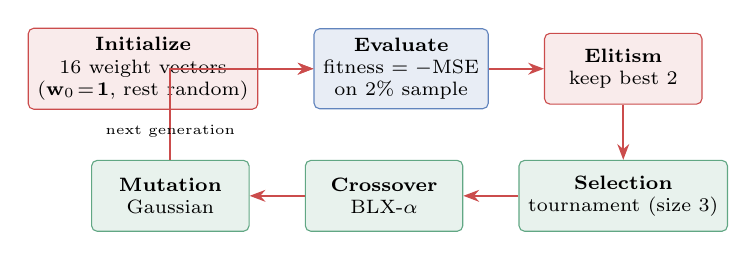
\begin{tikzpicture}[node distance=0.4cm and 0.7cm]
    \node[box] (init) {\textbf{Initialize}\\ 16 weight vectors\\ ($\mathbf w_0\!=\!\mathbf 1$, rest random)};
    \node[bluebox, right=of init] (eval) {\textbf{Evaluate}\\ fitness $=-$MSE\\ on 2\% sample};
    \node[box, right=of eval] (elite) {\textbf{Elitism}\\ keep best 2};
    \node[greenbox, below=0.7cm of elite] (sel) {\textbf{Selection}\\ tournament (size 3)};
    \node[greenbox, left=of sel] (cross) {\textbf{Crossover}\\ BLX-$\alpha$};
    \node[greenbox, left=of cross] (mut) {\textbf{Mutation}\\ Gaussian};

    \draw[flow] (init)--(eval);
    \draw[flow] (eval)--(elite);
    \draw[flow] (elite)--(sel);
    \draw[flow] (sel)--(cross);
    \draw[flow] (cross)--(mut);
    \draw[flow] (mut) |- (eval) node[pos=0.25, below, font=\tiny]{next generation};
  \end{tikzpicture}

  \vspace{0.3cm}
  \begin{columns}[T]
    \begin{column}{0.32\textwidth}
      \begin{block}{Selection}
        \scriptsize Pick 3 individuals at random; the one with best fitness becomes a parent.
        Repeat for the second parent.
      \end{block}
    \end{column}
    \begin{column}{0.32\textwidth}
      \begin{block}{Crossover (rate 0.8)}
        \scriptsize BLX-$\alpha$ blends two parents per gene (next slide).
      \end{block}
    \end{column}
    \begin{column}{0.32\textwidth}
      \begin{block}{Mutation (rate 0.4)}
        \scriptsize Perturb 1--3 genes by $\mathcal N(0,0.25)$; clamp to be positive.
      \end{block}
    \end{column}
  \end{columns}
\end{frame}

\begin{frame}{How we get a new solution: BLX-$\alpha$ crossover}
  \begin{columns}[T]
    \begin{column}{0.46\textwidth}
      For each gene $d$, given parents $p_1,p_2$, let
      $\text{lo}=\min(p_1,p_2)$, $\text{hi}=\max(p_1,p2)$, $I=\text{hi}-\text{lo}$.
      The child gene is drawn \alert{uniformly} from
      \[
        \big[\,\text{lo}-\alpha I,\;\; \text{hi}+\alpha I\,\big],\quad \alpha=0.5 .
      \]
      \begin{itemize}
        \item Children can lie \emph{between} parents \textbf{or slightly beyond} them
              (the $\alpha I$ margin) --- this gives exploration.
        \item Applied gene-by-gene, so each of the 8 weights is blended independently.
      \end{itemize}
      \begin{block}{Then mutation}
        With prob.\ 0.4, add Gaussian noise to 1--3 random genes, then clamp $\ge 0.05$.
        This is how a genuinely \textbf{new} weight vector appears.
      \end{block}
    \end{column}
    \begin{column}{0.54\textwidth}
      \centering
      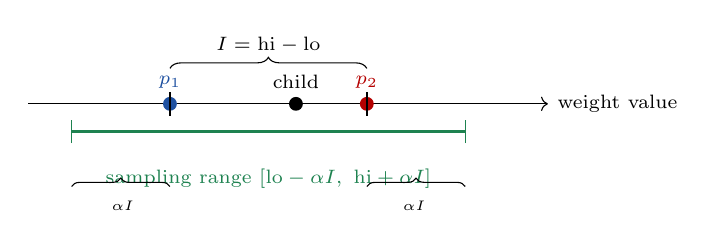
\begin{tikzpicture}[scale=1.0]
        % number line
        \draw[->] (-0.3,0)--(6.3,0) node[right,font=\scriptsize]{weight value};
        % parents
        \fill[accentblue] (1.5,0) circle (2.5pt) node[above=2pt,font=\scriptsize,accentblue]{$p_1$};
        \fill[ntnured]    (4.0,0) circle (2.5pt) node[above=2pt,font=\scriptsize,ntnured]{$p_2$};
        % interval lo..hi
        \draw[thick] (1.5,-0.15)--(1.5,0.15);
        \draw[thick] (4.0,-0.15)--(4.0,0.15);
        % extended interval
        \draw[accentgreen, very thick] (0.25,-0.35)--(5.25,-0.35);
        \draw[accentgreen] (0.25,-0.5)--(0.25,-0.2);
        \draw[accentgreen] (5.25,-0.5)--(5.25,-0.2);
        \node[accentgreen, font=\scriptsize, below] at (2.75,-0.7)
            {sampling range $[\text{lo}-\alpha I,\ \text{hi}+\alpha I]$};
        % I bracket
        \draw[decorate, decoration={brace, amplitude=4pt}] (1.5,0.45)--(4.0,0.45);
        \node[font=\scriptsize] at (2.75,0.75) {$I=\text{hi}-\text{lo}$};
        % alpha I margins
        \draw[decorate, decoration={brace, amplitude=3pt}] (0.25,-1.05)--(1.5,-1.05);
        \node[font=\tiny] at (0.9,-1.3){$\alpha I$};
        \draw[decorate, decoration={brace, amplitude=3pt}] (4.0,-1.05)--(5.25,-1.05);
        \node[font=\tiny] at (4.6,-1.3){$\alpha I$};
        % a sampled child
        \fill[black] (3.1,0) circle (2.5pt) node[above=2pt,font=\scriptsize]{child};
      \end{tikzpicture}

      \vspace{0.3cm}
      {\scriptsize One gene shown. The child is a random point in the green range; repeating
      for all 8 genes produces one offspring weight vector.}
    \end{column}
  \end{columns}
\end{frame}

\begin{frame}{What the GA learned (and why it generalizes)}
  \begin{columns}[T]
    \begin{column}{0.5\textwidth}
      Converged weights (train image \texttt{0003}, sampled MSE $72.82\!\to\!71.77$):
      \vspace{0.15cm}

      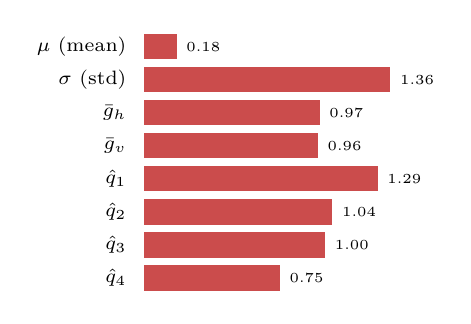
\begin{tikzpicture}[scale=1.0]
        \def\barh{0.32}
        \foreach \i/\name/\w [count=\y] in {
          1/$\mu$ (mean)/0.18, 2/$\sigma$ (std)/1.36, 3/$\bar g_h$/0.97,
          4/$\bar g_v$/0.96, 5/$\hat q_1$/1.29, 6/$\hat q_2$/1.04,
          7/$\hat q_3$/1.00, 8/$\hat q_4$/0.75}{
          \node[font=\scriptsize, left] at (0,-\y*0.42) {\name};
          \fill[ntnured!70] (0.1,-\y*0.42-\barh/2) rectangle (0.1+\w*2.3,-\y*0.42+\barh/2);
          \node[font=\tiny, right] at (0.1+\w*2.3,-\y*0.42) {\w};
        }
      \end{tikzpicture}
    \end{column}
    \begin{column}{0.5\textwidth}
      \begin{exampleblock}{The result matches theory exactly}
        \begin{itemize}
          \item \alert{$\mu$ smallest} (0.18): a mean mismatch is absorbed by offset $o$
                --- so it should barely count.
          \item \alert{$\sigma$ largest} (1.36): a contrast mismatch cannot be absorbed
                --- so it should count most.
          \item Ratio $\sigma/\mu \approx \mathbf{7.6\times}$.
        \end{itemize}
      \end{exampleblock}
      \begin{block}{Why one training image is enough}
        ``$\sigma$ drives the multiplicative contrast, $\mu$ is free'' is a property of the
        \textbf{affine model} (the formula for $s,o$), \emph{not} of any image. So the weights
        transfer --- and indeed they improve PSNR on \textbf{all 10} unseen test images.
      \end{block}
    \end{column}
  \end{columns}
\end{frame}

% ============================================================
\section{Experiments}
% ============================================================

\begin{frame}{Experimental setup and the four experiments}
  \begin{columns}[T]
    \begin{column}{0.5\textwidth}
      \begin{block}{Setup}
        \begin{itemize}
          \item 10 DIV2K images, $1024\times1024$, grayscale.
          \item $L\!=\!4$, domain $8$, stride $4$; CR $\approx 3.7{:}1$.
          \item FFE budget 800 per block (fair common axis).
          \item PSO methods: 5 runs each; FGDS deterministic.
          \item Significance: Wilcoxon signed-rank, $n\!=\!10$.
          \item GA trained on \texttt{0003} (held out).
        \end{itemize}
      \end{block}
    \end{column}
    \begin{column}{0.5\textwidth}
      \begin{exampleblock}{Four connected experiments}
        \begin{description}
          \item[E1] PSO / Memetic / FG-PSO / FGDS ($K{=}40$) --- shows the optimizer is
                    unnecessary.
          \item[E2] FGDS pairwise / KD-Tree / KD-Tree+GA ($K{=}80$) --- isolates the
                    speedup and the GA gain.
          \item[E3] $K\in\{5,..,160\}$ sweep --- finds the sweet spot.
          \item[E4] feature pool vs.\ \emph{random} pool ($K{=}80$) --- proves the features
                    matter.
        \end{description}
      \end{exampleblock}
    \end{column}
  \end{columns}
\end{frame}

\begin{frame}{E1: the optimizer is not the bottleneck}
  \begin{columns}[T]
    \begin{column}{0.48\textwidth}
      \centering
      \footnotesize
      \begin{tabular}{lrr}
        \toprule
        \textbf{Method} & \textbf{PSNR (dB)} & \textbf{Time (s)} \\
        \midrule
        PSO            & 28.87 & 1419.8 \\
        Memetic PSO    & 29.15 & 1317.2 \\
        FG-PSO ($K{=}40$) & 30.27 & 1268.8 \\
        \rowcolor{ntnured!12}
        \textbf{FGDS ($K{=}40$)} & \textbf{30.80} & \textbf{358.0} \\
        \bottomrule
      \end{tabular}

      \vspace{0.3cm}
      \begin{block}{Read it as a trail}
        \scriptsize
        LS helps (+0.28); feature pool helps more (+1.12);
        dropping PSO for exhaustive helps again (+0.53) --- with
        \textbf{$\sim$4$\times$ speedup} and no randomness.
      \end{block}
    \end{column}
    \begin{column}{0.52\textwidth}
      
\includegraphics[width=\linewidth]{images/convergence_average_exp1.png}

      {\scriptsize Feature-guided methods start 2--3 dB higher; FGDS saturates at
      $K\!\times\!8=320$ FFEs and stays on top.}
    \end{column}
  \end{columns}
\end{frame}

\begin{frame}{E2: KD-Tree gives the same quality, far faster ($+$ GA)}
  \begin{columns}[T]
    \begin{column}{0.5\textwidth}
      \centering
      \footnotesize
      \begin{tabular}{lrrr}
        \toprule
        \textbf{Variant} & \textbf{PSNR} & \textbf{CandSel(s)} & \textbf{MSE} \\
        \midrule
        Pairwise        & 31.21 & 179.57 & 56.27 \\
        KD-Tree         & 31.21 & \textbf{0.13} & 56.27 \\
        \rowcolor{accentgreen!12}
        KD-Tree $+$ GA  & \textbf{31.26} & 0.12 & \textbf{55.60} \\
        \bottomrule
      \end{tabular}
      \vspace{0.3cm}
      \begin{exampleblock}{Two clean results}
        \scriptsize
        \begin{itemize}
          \item KD-Tree $=$ pairwise in quality (identical neighbours), but candidate
                selection drops $179.6\,\text{s}\to 0.13\,\text{s}$ ($\sim$1390$\times$).
          \item GA weights add $+0.05$ dB on average, \textbf{positive on all 10 images},
                at zero encoding cost.
        \end{itemize}
      \end{exampleblock}
    \end{column}
    \begin{column}{0.5\textwidth}
      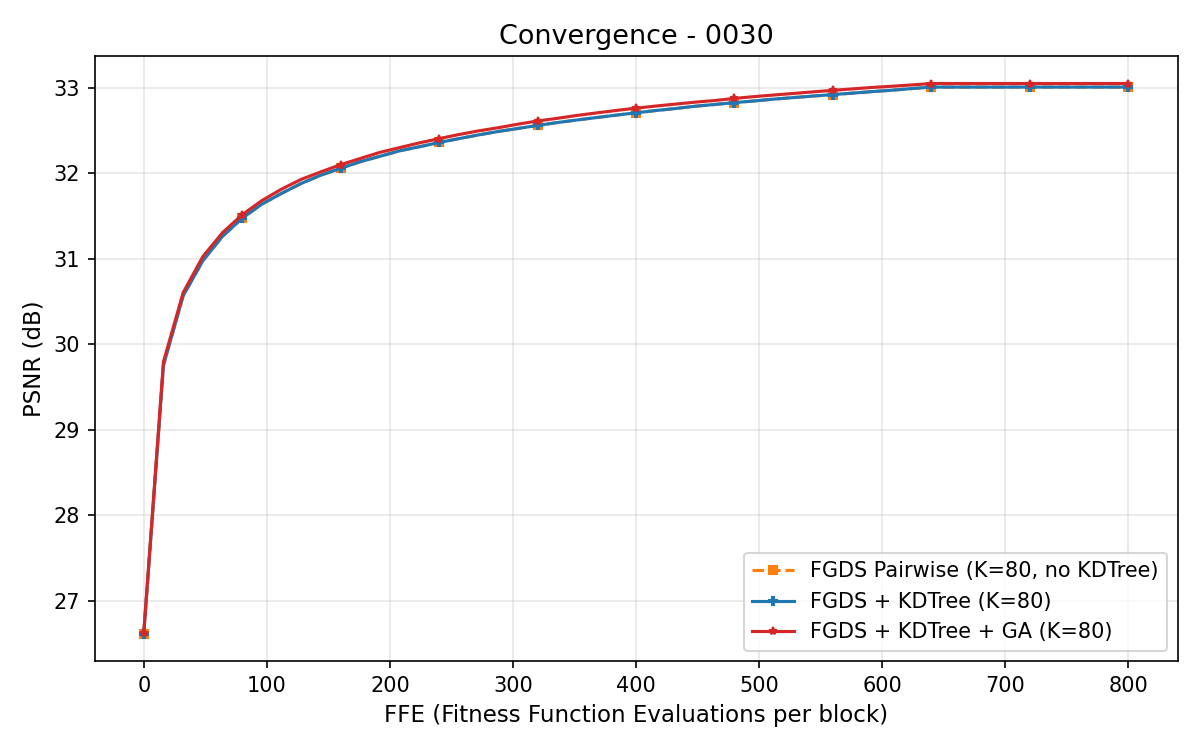
\includegraphics[width=\linewidth]{images/convergence_0030.png}

      {\scriptsize Image 0030: the three variants overlap almost perfectly (same neighbours);
      GA is marginally on top.}
    \end{column}
  \end{columns}
\end{frame}

\begin{frame}{E3: choosing the pool size $K$}
  \begin{columns}[T]
    \begin{column}{0.5\textwidth}
      \centering
      \footnotesize
      \begin{tabular}{rrrr}
        \toprule
        $K$ & \textbf{FFE} & \textbf{PSNR (dB)} & \textbf{Total (s)} \\
        \midrule
        5   & 40   & 29.18 & 51.6 \\
        10  & 80   & 29.80 & 95.7 \\
        20  & 160  & 30.33 & 183.6 \\
        40  & 320  & 30.80 & 360.9 \\
        \rowcolor{ntnured!12}
        80  & 640  & 31.21 & 712.9 \\
        160 & 1280 & 31.33 & 884.7 \\
        \bottomrule
      \end{tabular}
    \end{column}
    \begin{column}{0.5\textwidth}
      \begin{block}{Diminishing returns}
        \begin{itemize}
          \item PSNR climbs steadily up to $K=80$ (31.21 dB).
          \item $K=80\to160$: only \textbf{+0.12 dB} for $\sim$1.24$\times$ the time.
          \item $\Rightarrow$ the top-80 feature neighbours already contain essentially all
                useful domains.
        \end{itemize}
      \end{block}
      \begin{exampleblock}{Decision}
        Adopt \alert{$K=80$} as the sweet spot (used in E2 and E4). Even $K=40$ already beats
        every PSO baseline at a fraction of the time.
      \end{exampleblock}
    \end{column}
  \end{columns}
\end{frame}

\begin{frame}{E4: is it the features, or just a smaller pool?}
  \begin{columns}[T]
    \begin{column}{0.48\textwidth}
      \textbf{Control experiment.} Replace the feature-guided pool with a \alert{random}
      pool of the \emph{same} size ($K=80$), same exhaustive search, same FFEs. Only the
      \emph{selection} differs.
      \vspace{0.2cm}
      \begin{alertblock}{Result}
        \begin{itemize}
          \item FGDS-80: \textbf{31.21 dB} \quad vs.\quad Random-80: 27.96 dB
          \item Gap $=$ \textbf{+3.25 dB}, FGDS wins on \textbf{all 10} images.
        \end{itemize}
      \end{alertblock}
      A same-size random pool is far worse $\Rightarrow$ the quality comes from the
      \textbf{feature-guided selection}, not from shrinking the space alone. \emph{This is the
      core of our thesis.}
    \end{column}
    \begin{column}{0.52\textwidth}
      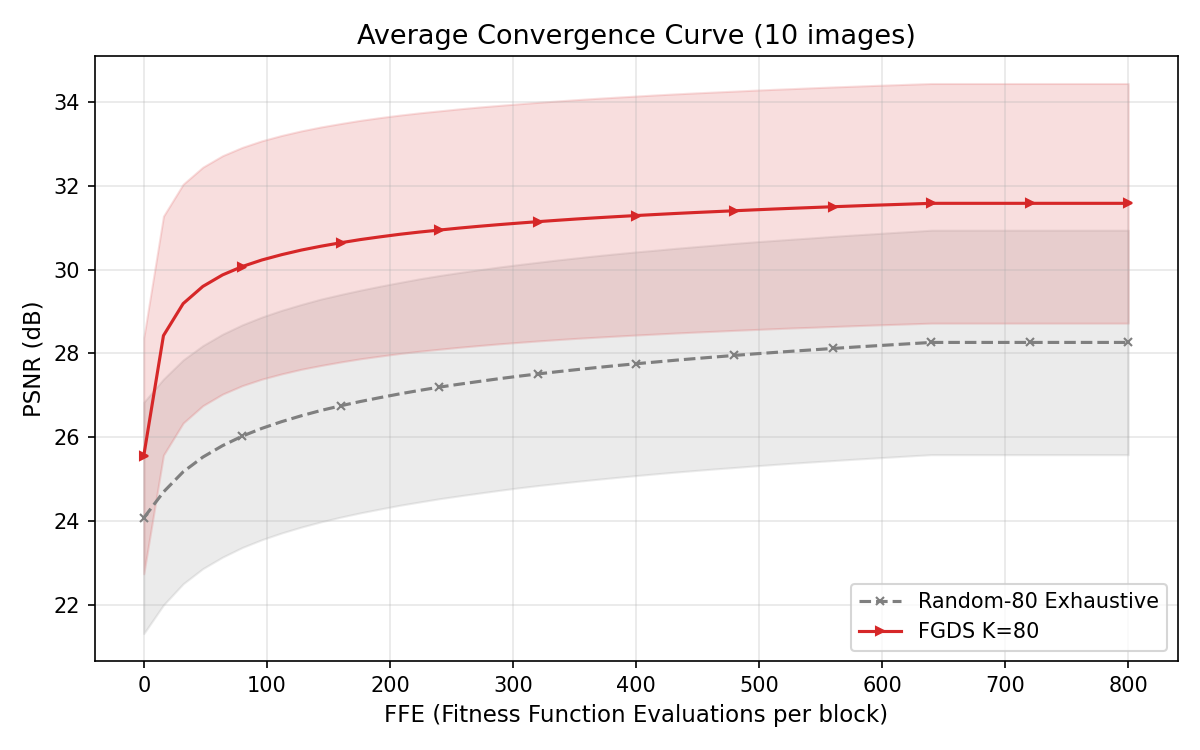
\includegraphics[width=\linewidth]{images/convergence_average_random.png}

      {\scriptsize At equal FFEs the feature-guided pool (red) dominates the random pool
      (gray) throughout by $\sim$3.25 dB.}
    \end{column}
  \end{columns}
\end{frame}

\begin{frame}{Statistical significance and a visual example}
  \begin{columns}[T]
    \begin{column}{0.5\textwidth}
      \centering
      \footnotesize
      \textbf{Wilcoxon signed-rank (PSNR, $n=10$)}
      \vspace{0.1cm}
      \begin{tabular}{lrr}
        \toprule
        \textbf{Comparison} & $\Delta$PSNR & $p$ \\
        \midrule
        FGDS vs.\ PSO         & $+1.93$ & $<0.01$ \\
        FGDS vs.\ Memetic PSO & $+1.65$ & $<0.01$ \\
        FGDS vs.\ FG-PSO      & $+0.53$ & $<0.01$ \\
        FGDS$+$GA vs.\ FGDS   & $+0.05$ & $<0.01$ \\
        FGDS-80 vs.\ Random-80& $+3.25$ & $<0.01$ \\
        \bottomrule
      \end{tabular}

      \vspace{0.2cm}
      {\scriptsize FGDS wins every paired image in every comparison
      ($W^+\!=\!55$, exact $p=1/2^{10}\approx0.001$).}
    \end{column}
    \begin{column}{0.5\textwidth}
      \centering
      \begin{columns}[T]
        \begin{column}{0.5\textwidth}
          \centering
          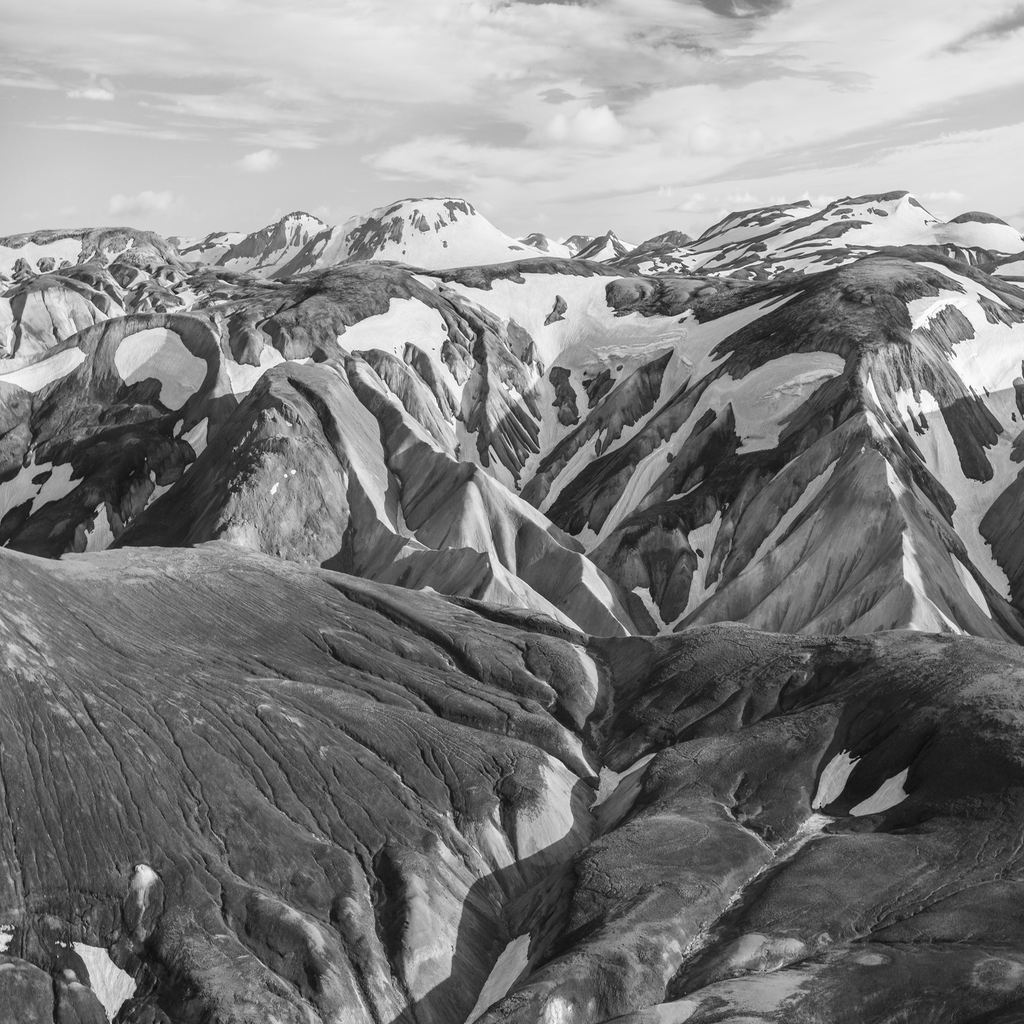
\includegraphics[width=\linewidth]{images/0030_original.png}\\
          {\scriptsize Original (0030)}
        \end{column}
        \begin{column}{0.5\textwidth}
          \centering
          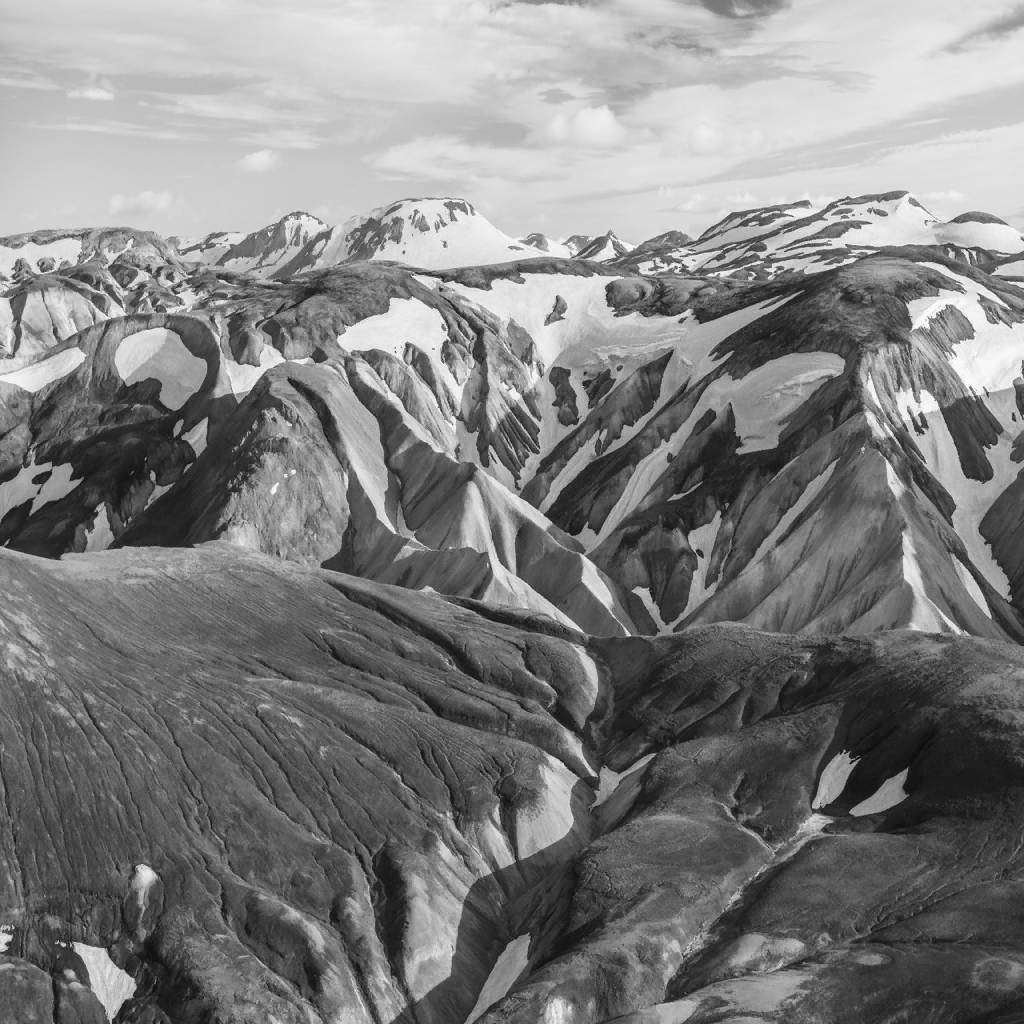
\includegraphics[width=\linewidth]{images/0030_fgds_ga_reconstructed.png}\\
          {\scriptsize FGDS$+$GA, 32.73 dB}
        \end{column}
      \end{columns}
      \vspace{0.2cm}
      {\scriptsize Ridges, snow boundaries, and sky gradients are preserved at
      CR $\approx 3.7{:}1$.}
    \end{column}
  \end{columns}
\end{frame}

% ============================================================
\section{Conclusion}
% ============================================================

\begin{frame}{Conclusion}
  \begin{block}{What we showed}
    \begin{itemize}
      \item For high-resolution FIC, the bottleneck is the \textbf{search space}, not the
            optimizer. A feature pool of 80 domains, searched exhaustively, beats PSO over
            $5\times10^5$ candidates by $\sim$1.9 dB.
      \item Once the pool is small, \textbf{exhaustive search dominates PSO} --- so we remove
            the metaheuristic matcher entirely.
      \item A \textbf{KD-Tree} builds the pool $\sim$1390$\times$ faster than pairwise, with
            identical quality.
      \item A \textbf{GA} learns, offline and once, how much each feature matters; the learned
            weights ($\sigma\!\gg\!\mu$) follow from the affine model and transfer to all images.
    \end{itemize}
  \end{block}
  \begin{exampleblock}{Our contribution}
    We move the heuristic from block \textbf{matching} to feature-guided block
    \textbf{selection}. Result: \textbf{+1.7--3.2 dB} over PSO, \textbf{$\sim$4$\times$ faster},
    all gains significant at $p<0.01$; a random-pool control attributes \textbf{+3.25 dB}
    specifically to the feature-guided selection.
  \end{exampleblock}
\end{frame}

\begin{frame}{Thank you}
  \centering
  \vspace{0.8cm}
  {\Large\color{ntnured}\textbf{Feature-Guided Domain Selection}}\\[2pt]
  {\large for Fast Fractal Image Compression}\\[0.6cm]
  Zhen-Rong Wu \quad Darrin Lin \quad Liang-Yun Ko\\[0.3cm]
  {\small National Taiwan Normal University}\\[0.6cm]
  {\small Source code: \texttt{github.com/noyapoyo/pso-ma-fic}}\\[0.8cm]
  \begin{block}{Take-away}
    \centering
    When a metaheuristic struggles on a combinatorial problem, apply it to the
    \emph{design of the search space} --- not to the search itself.
  \end{block}
\end{frame}

\end{document}